%==============================================================================
%  SwiftDrop --- Technical Project Report
%  Build:  tectonic -X compile SwiftDrop_Project_Report.tex
%  Images: ../docs/diagrams/  (18 verified architecture diagrams)
%==============================================================================
\documentclass[11pt,a4paper,oneside,openany]{report}

%================================================================== packages
\usepackage[T1]{fontenc}
\usepackage[utf8]{inputenc}
\usepackage{lmodern}
\usepackage[a4paper,top=2.6cm,bottom=2.6cm,left=2.6cm,right=2.4cm]{geometry}
\usepackage{graphicx}
\usepackage{booktabs}
\usepackage{longtable}
\usepackage{array}
\usepackage{xcolor}
\usepackage{fancyhdr}
% (rotation uses \rotatebox from graphicx — no floating-rotation package needed)
\usepackage[font=small,labelfont=bf,textfont=it]{caption}
\usepackage{enumitem}
\usepackage{titlesec}
\usepackage{tcolorbox}
\usepackage{float}
\usepackage{ragged2e}
\usepackage{amssymb}
\usepackage{microtype}
\usepackage[hidelinks,bookmarksnumbered]{hyperref}

% Let long \texttt tokens and tight columns break rather than overflow
\emergencystretch=3em
\hbadness=10000
\hfuzz=4pt

% Never stretch a short page to full height, and never let a float get deferred
% onto a page of its own — both are the usual sources of blank pages.
\raggedbottom
\renewcommand{\topfraction}{0.95}
\renewcommand{\bottomfraction}{0.95}
\renewcommand{\textfraction}{0.05}
\renewcommand{\floatpagefraction}{0.85}
\setcounter{topnumber}{3}
\setcounter{bottomnumber}{2}
\setcounter{totalnumber}{5}

\graphicspath{{../docs/diagrams/}}

%======================================================== status label macros
% Monochrome throughout: status is carried by the word itself, not by colour.
\newcommand{\Impl}{\textbf{Implemented}}
\newcommand{\Partial}{\textbf{Partial}}
\newcommand{\Planned}{\textbf{Planned}}
\newcommand{\code}[1]{\texttt{\small #1}}

%============================================================ title page data
\newcommand{\UniversityName}{University of Moratuwa}
\newcommand{\FacultyName}{Faculty of Information Technology}
\newcommand{\ModuleName}{Enterprise Application Development (IN3101)}
\newcommand{\RepoUrl}{https://github.com/Kevin200307/enterpriseProject.git}

%============================================================== page styling
\pagestyle{fancy}
\fancyhf{}
\setlength{\headheight}{14pt}
\renewcommand{\headrulewidth}{0.4pt}
\renewcommand{\footrulewidth}{0pt}
\fancyhead[L]{\small SwiftDrop Technical Project Report}
\fancyhead[R]{\small\leftmark}
\fancyfoot[C]{\small\thepage}
\fancypagestyle{plain}{\fancyhf{}\fancyfoot[C]{\small\thepage}\renewcommand{\headrulewidth}{0pt}}

\renewcommand{\chaptermark}[1]{\markboth{\thechapter.\ #1}{}}

\titleformat{\chapter}[display]
  {\normalfont\huge\bfseries}
  {\Large\chaptertitlename\ \thechapter}{10pt}{\Huge}
\titlespacing*{\chapter}{0pt}{-20pt}{26pt}
\titleformat{\section}{\normalfont\Large\bfseries}{\thesection}{1em}{}
\titleformat{\subsection}{\normalfont\large\bfseries}{\thesubsection}{1em}{}

\captionsetup[figure]{skip=8pt}
\setlist{itemsep=2pt,parsep=0pt,topsep=4pt}

% Callout box, monochrome
\newtcolorbox{factbox}[1][]{
  colback=white, colframe=black, boxrule=0.5pt, arc=2pt,
  left=8pt, right=8pt, top=6pt, bottom=6pt, #1}

% Standard figure helper: auto-scaled, never taller than the page
\newcommand{\diagram}[3]{%
  \begin{figure}[H]\centering
  \includegraphics[width=\linewidth,height=0.78\textheight,keepaspectratio]{#1}
  \caption{#2}\label{#3}\end{figure}}

\begin{document}

%==============================================================================
\begin{titlepage}
\centering
\vspace*{1.2cm}
{\Large\scshape \UniversityName\par}
\vspace{0.4cm}
{\large \FacultyName\par}
\vspace{2.0cm}
{\rule{\linewidth}{1.2pt}}\par
\vspace{1.0cm}
{\Huge\bfseries SwiftDrop\par}
\vspace{0.5cm}
{\LARGE Cloud-Native Parcel Delivery \&\\[6pt] Courier Management Platform\par}
\vspace{0.8cm}
{\large\itshape Technical Project Report\par}
\vspace{1.0cm}
{\rule{\linewidth}{1.2pt}}\par
\vspace{2.0cm}

{\large\textbf{Module}\par}
\vspace{0.25cm}
{\large \ModuleName\par}

\vspace{1.2cm}
{\large\textbf{Group 4}\par}

\vspace{1.4cm}
{\large\textbf{Project Repository}\par}
\vspace{0.25cm}
{\small\url{\RepoUrl}\par}

\vfill
\end{titlepage}

%==============================================================================
\chapter*{Declaration and Team Composition}
\addcontentsline{toc}{chapter}{Declaration and Team Composition}
\markboth{Declaration and Team Composition}{}

This report documents the design and implementation of \textbf{SwiftDrop}, a distributed
parcel delivery and courier management platform developed by a ten-member engineering team.
Every architectural claim, diagram, table and figure in this document has been verified
directly against the project source code.

\vspace{0.6cm}
\begin{center}
\small
\begin{tabular}{@{}p{2.2cm}p{4.3cm}p{4.2cm}p{3.4cm}@{}}
\toprule
\textbf{Index No.} & \textbf{Member} & \textbf{Area of Ownership} & \textbf{GitHub} \\
\midrule
234021D & Arangala A. P.        & Identity \& Authentication   & \code{@AmandiArangala} \\
        & Kevin Gaveshana       & API Gateway \& Edge Platform & \code{@Kevin200307} \\
234127H & M.A.P.M. Mallawasekara& Pricing \& Zone Management   & \code{@Pavindu11} \\
234087H & L. P. Ishadi          & Parcel Booking \& Lifecycle  & \code{@LP-Ishadi} \\
234149C & Methsara              & Dispatch \& Courier Workload & \code{@Dimeshmethsara} \\
        & Charithma Dassanayake & Merchant API \& Webhooks     & \code{@CDDassanayake} \\
234009A & Maheesha Paboth       & Live Tracking \& WebSockets  & \code{@MaheeshaPaboth} \\
234208H & Thranjaya S. J. K.    & Notification Pipeline        & \code{@thirsturn} \\
234234H & R.K.T.P. Wijerathna   & AI Assistant \& Tooling      & \code{@Prabhashwara2003} \\
234035A & K.G.T. Buddhima       & Frontend SPA \& System Design& \code{@ThanojBuddhima} \\
\bottomrule
\end{tabular}
\end{center}

%==============================================================================
\tableofcontents

%==============================================================================
\chapter{Introduction and Project Context}

\section{Background}
The rapid growth of digital commerce has made agile, reliable last-mile logistics essential to
modern trade. Traditional courier operations still rely on disconnected records, manual dispatch
ledgers and monolithic backends that create operational silos, offer no live visibility, and
degrade under peak demand.

\textbf{SwiftDrop} is a cloud-native, distributed parcel delivery and courier management platform
that unifies parcel booking, zone-based pricing, courier dispatch, real-time tracking,
multi-channel notification and commercial merchant integration. The platform additionally
includes an \textbf{AI assistant service} built on Spring AI, which exposes read-oriented domain
tools to a large language model so users can query the system in natural language.

\section{Problem Statement}
Contemporary logistics platforms exhibit several recurring deficiencies, each of which shaped a
design decision in SwiftDrop.

\begin{enumerate}[leftmargin=*]
\item \textbf{Opaque transit visibility.} Batch-updated records do not reflect instantaneous
transit checkpoints. Customers experience uncertainty about delivery windows, and couriers lack a
standardised mechanism to capture tamper-evident proof of delivery at the doorstep.

\item \textbf{Inflexible, manual pricing.} Coarse rate cards fail to accommodate multi-tier
geographic zones, parcel size bands, weight allowances and express service tiers, causing revenue
leakage for operators and unexpected charges for customers.

\item \textbf{Sub-optimal dispatch and workload imbalance.} Ad-hoc manual assignment leaves
dispatchers without unified visibility of courier capacity, producing delayed pickups, uneven
workload and elevated failure rates.

\item \textbf{Friction in B2B partner integration.} Merchants needing programmatic, high-volume
shipping are hindered by proprietary APIs lacking self-service key provisioning, scoped
authorisation and resilient webhook pipelines.

\item \textbf{Monolithic fragility.} Shared-database contention means high-volume read traffic
(thousands of concurrent tracking lookups) degrades critical transactional paths, and a failure in
an auxiliary subsystem can cascade across the whole application.

\item \textbf{Manual operational overhead.} Routine enquiries - tracking lookups, fee quotations,
delivery history - consume human support capacity that a natural-language interface can absorb.
\end{enumerate}

\section{Objectives}
The SwiftDrop platform was designed around four dimensions: functional capability, AI assistant
capability, architectural standards, and security and quality assurance.

\subsection{Functional Objectives}
\begin{itemize}[leftmargin=*]
\item Provide a self service booking portal that calculates shipping tariffs in real time from the
origin and destination zones, parcel size band, weight and service speed.
\item Extend tariff calculation to volumetric parcel dimensions and negotiated merchant volume
discounts.
\item Deliver dedicated, responsive web portals for Customers, Merchants, Couriers, Dispatchers and
Administrators.
\item Implement push based shipment tracking using STOMP over WebSockets, with Server Sent Events
and polling as progressive fallbacks.
\item Guarantee asynchronous transactional notification on every parcel lifecycle milestone,
addressed to both the sender and the recipient.
\item Support email and SMS as independently configurable notification channels governed by per
user preferences.
\item Supply a secured partner REST API with scoped API keys and outbound HMAC signed webhooks
backed by exponential backoff retry.
\end{itemize}

\subsection{AI Assistant Objectives}
\begin{itemize}[leftmargin=*]
\item Implement a tool calling assistant over the domain services using Spring AI, so the platform
can be queried in natural language.
\item Expose conversational fee estimation, parcel tracking and delivery history as callable tools.
\item Extend the assistant with write capable tools for parcel booking, dispatch allocation and
merchant operations such as key provisioning and webhook retry.
\item Publish the same tool surface over the Model Context Protocol so external clients can consume
it.
\item Stream the assistant's tool invocations to the client over Server Sent Events for full
operational transparency.
\item Filter the active tool set at runtime against the caller's granted authorities so the
assistant never exceeds the user's own permissions.
\end{itemize}

\subsection{Architectural Objectives}
\begin{itemize}[leftmargin=*]
\item Partition the platform into autonomous Spring Boot microservices aligned with
Domain Driven Design bounded contexts.
\item Enforce database per service encapsulation, eliminating cross service joins and shared
database locks.
\item Deploy a reactive Spring Cloud Gateway as the single perimeter ingress, responsible for
routing, CORS, token validation, rate limiting and circuit breaking.
\item Decouple domain state changes through a RabbitMQ topic exchange to achieve fault tolerance
and eventual consistency across downstream consumers.
\item Containerise every service and backing dependency, orchestrated locally through Docker
Compose.
\item Orchestrate the platform on Kubernetes through an umbrella Helm chart covering deployments,
services, config maps, secrets and ingress.
\item Scale the edge and tracking workloads independently using Kubernetes Horizontal Pod
Autoscalers.
\end{itemize}

\subsection{Security and Quality Objectives}
\begin{itemize}[leftmargin=*]
\item Implement RSA 2048 bit RS256 JSON Web Tokens with RFC 7517 JWKS discovery, enabling stateless
downstream validation.
\item Integrate Google OAuth 2.0 with Proof Key for Code Exchange for federated sign in.
\item Rotate refresh tokens on every use and revoke the entire token family on replay detection.
\item Verify core business rules and state machines through unit testing with JUnit 5 and Mockito.
\item Exercise repository and messaging behaviour against real PostgreSQL and RabbitMQ instances
using Testcontainers.
\item Assert the role based authorisation matrix so unauthorised roles are provably refused.
\item Cover the critical user journeys with end to end browser smoke tests.
\end{itemize}

\section{Technology Stack}
\begin{center}
\small
\begin{longtable}{@{}p{3.9cm}p{10.4cm}@{}}
\toprule
\textbf{Layer} & \textbf{Technology} \\
\midrule
\endfirsthead
\toprule
\textbf{Layer} & \textbf{Technology} \\
\midrule
\endhead
Frontend application & React 18.3, TypeScript, Vite, Tailwind CSS, TanStack React Query, React
Router \\
\addlinespace
Edge gateway / BFF & Spring Cloud Gateway (Project Reactor, Netty), Redis token-bucket rate
limiting, Resilience4j circuit breakers \\
\addlinespace
Backend microservices & Java 21, Spring Boot 4.1.1, Spring Security, Spring Data JPA, Jakarta Bean
Validation \\
\addlinespace
Persistence & PostgreSQL on Neon Cloud - \emph{one database per service} (six databases),
schema-managed by Flyway with \code{ddl-auto: validate} \\
\addlinespace
Cache and projection & Redis 7 - rate-limit buckets, login throttling, and the entire
tracking read projection \\
\addlinespace
Asynchronous broker & RabbitMQ 3 - topic exchange \code{parcel.events}, dead-letter exchange
\code{swiftdrop.dlx} \\
\addlinespace
Object storage & MinIO (S3-compatible) - proof-of-delivery photographs. PDF receipts are
generated on demand and are not stored \\
\addlinespace
Mail transport & Mailpit for local development; SMTP in deployed environments \\
\addlinespace
AI assistant & Spring AI with an OpenAI-compatible model provider \\
\addlinespace
Local orchestration & Docker Compose (all services plus backing infrastructure) \\
\addlinespace
Kubernetes orchestration & Umbrella Helm chart covering deployments, services, config maps, secrets and ingress \\
\bottomrule
\caption{Verified technology stack}\label{tab:stack}
\end{longtable}
\end{center}

%==============================================================================
\chapter{Requirements and Use Case Modelling}

\section{Actors and Authorisation Boundaries}
Authorisation is role-based. The five roles are declared once in a shared enumeration
(\code{contracts.domain.Role}) and carried in the \code{roles} claim of every access token, so the
actors below are the system's real authorisation boundaries rather than an analyst's abstraction.

\begin{center}
\small
\begin{tabular}{@{}llp{8.4cm}@{}}
\toprule
\textbf{Actor} & \textbf{Role} & \textbf{Capability boundary} \\
\midrule
Guest       & -           & Rate-limited public tracking lookup only; the sole capability
available without authentication \\
\addlinespace
Customer    & \code{CUSTOMER}   & Estimate fees, book deliveries, track parcels, download
receipts, manage notification preferences \\
\addlinespace
Merchant    & \code{MERCHANT}   & Granted only after administrator approval. Console access, API
key issuance, order placement, webhook configuration \\
\addlinespace
Courier     & \code{COURIER}    & Inspect assigned manifest, execute guarded status transitions,
capture photographic proof, record failure reasons \\
\addlinespace
Dispatcher  & \code{DISPATCHER} & Dispatch queue, courier workload, assignment and unassignment,
courier roster management \\
\addlinespace
Administrator & \code{ADMIN}    & Generalises Dispatcher; adds merchant approval, user and role
administration, zone and pricing configuration, notification audit \\
\bottomrule
\end{tabular}
\captionof{table}{System actors and authorisation boundaries}\label{tab:actors}
\end{center}

A merchant's \emph{backend system} is a second, non-human actor that authenticates with a scoped
API key rather than a user session.

\section{Use Case Specifications}
\begin{description}[leftmargin=1.4cm,style=nextline]
\item[Customer] Register; sign in with password or Google; estimate fee; book delivery; view
deliveries; track parcel; download receipt; cancel delivery; manage notification preferences;
apply to become a merchant.
\item[Merchant] Register organisation; await approval; create order through the console; create
order through the REST API; list and inspect orders; issue, list and revoke API keys; configure
webhook endpoint; inspect and replay webhook deliveries.
\item[Courier] View daily manifest; mark picked up, in transit and out for delivery; upload proof
of delivery; mark delivered; record failure with mandatory reason; reattempt a failed delivery.
\item[Dispatcher / Admin] Monitor dispatch queue; inspect courier workload; request assignment
suggestion; assign and unassign parcels; manage courier roster. Administrators additionally
approve merchants, manage users and roles, configure zones and pricing, and audit notifications.
\end{description}

\section{Use Case Diagrams}
\diagram{uc-00-system-overview.png}{System-level use case overview showing all actors, the
generalisation of \code{DISPATCHER} by \code{ADMIN}, and the capabilities shared across
roles}{fig:uc00}

\diagram{uc-01-customer.png}{Customer use cases. Booking \emph{includes} fee estimation because
the server re-quotes the price during booking rather than trusting the browser}{fig:uc01}

\diagram{uc-02-merchant.png}{Merchant use cases, distinguishing the human console path from the
server-to-server REST API path authenticated by a scoped API key}{fig:uc02}

\diagram{uc-03-courier.png}{Courier use cases. Every transition is guarded; marking a parcel
delivered \emph{includes} uploading proof of delivery}{fig:uc03}

\diagram{uc-04-dispatcher.png}{Dispatcher and administrator use cases, with the administrator-only
region shaded}{fig:uc04}

%==============================================================================
\chapter{System Architecture}

\section{Architectural Style and Justification}
SwiftDrop is built as \textbf{microservices behind an API gateway that also serves as a
backend-for-frontend}, with a strict three-layer structure inside every service.

The boundaries were derived from the domain, not from the technical layering: each service owns a
capability that changes for its own reasons. Pricing rules change when commercial terms change;
the parcel lifecycle changes when operations change; notification channels change when a provider
changes. There is no ``controller service'' or ``database service''.

\begin{enumerate}[leftmargin=*]
\item \textbf{Team independence.} Ten engineers developed and released their domains without code
contention.
\item \textbf{Blast-radius containment.} A spike in public tracking traffic or a failure in the
notification pipeline does not affect booking or authentication.
\item \textbf{Storage fit per context.} Tracking needs a fast, expiring, read-optimised projection
and uses Redis with a time-to-live, which would be awkward to justify inside a shared relational
schema.
\item \textbf{Independent scaling.} Read-heavy tracking and write-heavy booking scale on different
curves.
\end{enumerate}

\subsection{Honest Cost of This Choice}
A modular monolith with the same internal boundaries would have been a defensible - arguably
better - choice at this stage, and the costs microservices imposed are visible in the codebase.

\begin{center}
\small
\begin{tabular}{@{}p{4.6cm}p{9.6cm}@{}}
\toprule
\textbf{Cost} & \textbf{Where it appears} \\
\midrule
No cross-service transactions & Creating a merchant order writes to two databases through an HTTP
call; consistency is recovered with a transactional outbox, deterministic idempotency keys and
compensating reads \\
\addlinespace
User-visible eventual consistency & The dispatch board and tracking page are event-fed
projections; they are correct eventually and the interface must tolerate the gap \\
\addlinespace
Duplicated cross-cutting config & Every service repeats JWT decoder and resource-server setup; a
change to token validation is an eight-service change \\
\addlinespace
Contracts not compiler-checked & One service writes a JWT claim as \code{merchantId} while three
others read \code{merchant\_id} (Section~\ref{sec:defects}); in a single codebase this is a
compile error \\
\addlinespace
Operational surface & Six databases, a broker, Redis, an object store and a mail server must all
run before the system works end to end \\
\bottomrule
\end{tabular}
\captionof{table}{Costs incurred by the microservices decision}\label{tab:microcost}
\end{center}

The mitigation applied is a shared contracts module holding event schemas, shared enumerations and
error codes, with golden-file tests pinning the JSON shapes. It narrows the gap without closing it.

\section{Layered Topology}
The platform is organised into four layers.

\begin{description}[leftmargin=1.2cm,style=nextline]
\item[Presentation] A React single-page application. It holds no business rules - route guards
mirror server roles for user experience only, and every decision is re-made server-side. The
access token is held in memory, never in browser storage.
\item[Edge] Spring Cloud Gateway on WebFlux: the only publicly reachable component and the single
place implementing JWT validation (issuer and audience), CORS, security headers, Redis
token-bucket rate limiting, Resilience4j circuit breakers, request-id propagation and identity
header injection. Internal routes are denied outright at the edge.
\item[Business logic] Eight services, each owning a bounded context, each internally layered as
\code{api} $\rightarrow$ \code{service} $\rightarrow$ \code{repository} $\rightarrow$
\code{domain}. Dependencies point inward only; controllers carry no business rules and entities
never leave the service layer.
\item[Data] Six PostgreSQL databases, Redis, RabbitMQ and MinIO.
\end{description}

\diagram{arch-01-layers.png}{Layered architecture showing the presentation, edge, business-logic
and data layers, with synchronous calls solid and event flow dashed}{fig:arch01}

\diagram{arch-02-deployment.png}{Deployment topology: container boundaries, host port mappings and
external dependencies}{fig:arch02}

\section{Service Inventory}
\begin{center}
\small
\begin{longtable}{@{}p{3.5cm}p{10.8cm}@{}}
\toprule
\textbf{Service} & \textbf{Responsibility} \\
\midrule
\endfirsthead
\toprule
\textbf{Service} & \textbf{Responsibility} \\
\midrule
\endhead
gateway & Edge routing, JWT validation, CORS, rate limiting, circuit breaking, identity header
injection, aggregated API documentation \\
\addlinespace
identity-service & Registration, login, Google OIDC, RS256 token issuance, JWKS publication,
refresh rotation, role administration \\
\addlinespace
parcel-service & Parcel aggregate, booking, guarded state machine, proof upload, PDF receipts,
transactional outbox \\
\addlinespace
pricing-service & Zones, city resolution, temporal pricing rules, Strategy-based fee engine \\
\addlinespace
dispatch-service & Courier roster, dispatch queue projection, assignment commands, workload
accounting \\
\addlinespace
merchant-service & Merchant onboarding and approval, API key lifecycle, order ingestion, signed
outbound webhooks with retry \\
\addlinespace
tracking-service & Privacy-reduced read projection in Redis; STOMP and SSE push \\
\addlinespace
notification-service & Event-driven email and SMS dispatch, per-user preferences, delivery log,
retry scheduler \\
\addlinespace
ai-assistant-service & Stateless conversational assistant exposing read-oriented domain tools over
SSE \\
\bottomrule
\caption{Service inventory and responsibilities}\label{tab:services}
\end{longtable}
\end{center}

%==============================================================================
\chapter{Database and Entity-Relationship Modelling}

\section{Database-per-Service}
SwiftDrop implements database-per-service strictly. Six services own a PostgreSQL database each;
tracking-service holds its projection entirely in Redis, and ai-assistant-service has no
persistence at all.

The consequence that shapes the whole model is that \textbf{no service holds a foreign key into
another service's database}. Relationships crossing a service boundary exist only as UUID columns
enforced in application code. The identity \code{users.id} column is the most-referenced value in
the system - thirteen columns across four other databases point at it - and it has no inbound
foreign keys whatsoever.

\begin{factbox}
\textbf{Diagram convention.} A solid line is a real foreign key enforced by PostgreSQL. A dashed
line is a cross-database logical reference enforced only by application code.
\end{factbox}

\section{The 24-Table Domain Model}
\begin{center}
\small
\begin{longtable}{@{}p{3.4cm}p{2.6cm}p{8.3cm}@{}}
\toprule
\textbf{Service} & \textbf{Database} & \textbf{Tables} \\
\midrule
\endfirsthead
\toprule
\textbf{Service} & \textbf{Database} & \textbf{Tables} \\
\midrule
\endhead
identity-service & \code{identity\_db} & \code{users}, \code{roles}, \code{user\_roles},
\code{refresh\_tokens} \\
\addlinespace
parcel-service & \code{parcel\_db} & \code{parcels}, \code{parcel\_status\_history},
\code{delivery\_proofs}, \code{parcel\_outbox}, \code{parcel\_assignment\_commands} \\
\addlinespace
merchant-service & \code{merchant\_db} & \code{merchants}, \code{api\_keys},
\code{oauth\_clients}, \code{merchant\_orders}, \code{webhook\_deliveries} \\
\addlinespace
dispatch-service & \code{dispatch\_db} & \code{couriers}, \code{dispatch\_parcels},
\code{assignments}, \code{assignment\_commands}, \code{processed\_events} \\
\addlinespace
pricing-service & \code{pricing\_db} & \code{zones}, \code{zone\_cities}, \code{pricing\_rules} \\
\addlinespace
notification-service & \code{notification\_db} & \code{notifications},
\code{notification\_preferences} \\
\addlinespace
tracking-service & Redis only & \code{tracking:parcel:*}, \code{tracking:timeline:*}
(90-day time-to-live) \\
\addlinespace
ai-assistant-service & None & In-memory conversations, 24-hour expiry \\
\bottomrule
\caption{Table ownership across the six service databases}\label{tab:tables}
\end{longtable}
\end{center}

Points worth drawing out:

\begin{itemize}[leftmargin=*]
\item \textbf{Role-based access control} uses the classic three-table design. Role identifiers are
the enumeration names themselves, so a token's \code{roles} claim maps directly onto rows.
\item \textbf{\code{parcels} snapshots its fee.} Re-reading a parcel years later yields the price
actually charged, not what current rules would produce.
\item \textbf{\code{parcel\_status\_history} is an append-only audit trail} recording the
from-status, to-status, acting user, and an optional proof or failure reason for every transition.
\item \textbf{\code{couriers.id} is not \code{users.id}.} A courier has a dispatch-local surrogate
key, and \code{parcels.assignee\_id} points at the \emph{user}, so joining a parcel to a courier
always passes through the user identifier.
\item \textbf{Pricing is temporal.} Each rule carries an effective period, and a database trigger
forbids overlapping active periods for the same route and size band.
\end{itemize}

\section{Entity-Relationship Diagrams}
\diagram{er-01-core.png}{Core domain model covering users, roles, merchants, parcels, status
history, couriers, zones and pricing}{fig:er01}

\diagram{er-03-ownership.png}{Data ownership map: which service owns which tables, and every
logical reference that crosses a database boundary}{fig:er03}

% Portrait page, rotated diagram. Deliberately NOT a float: a float this large gets
% deferred to a page of its own and leaves a blank page behind it.
\clearpage
\begin{center}
\rotatebox{90}{%
  \begin{minipage}{0.90\textheight}
  \centering
  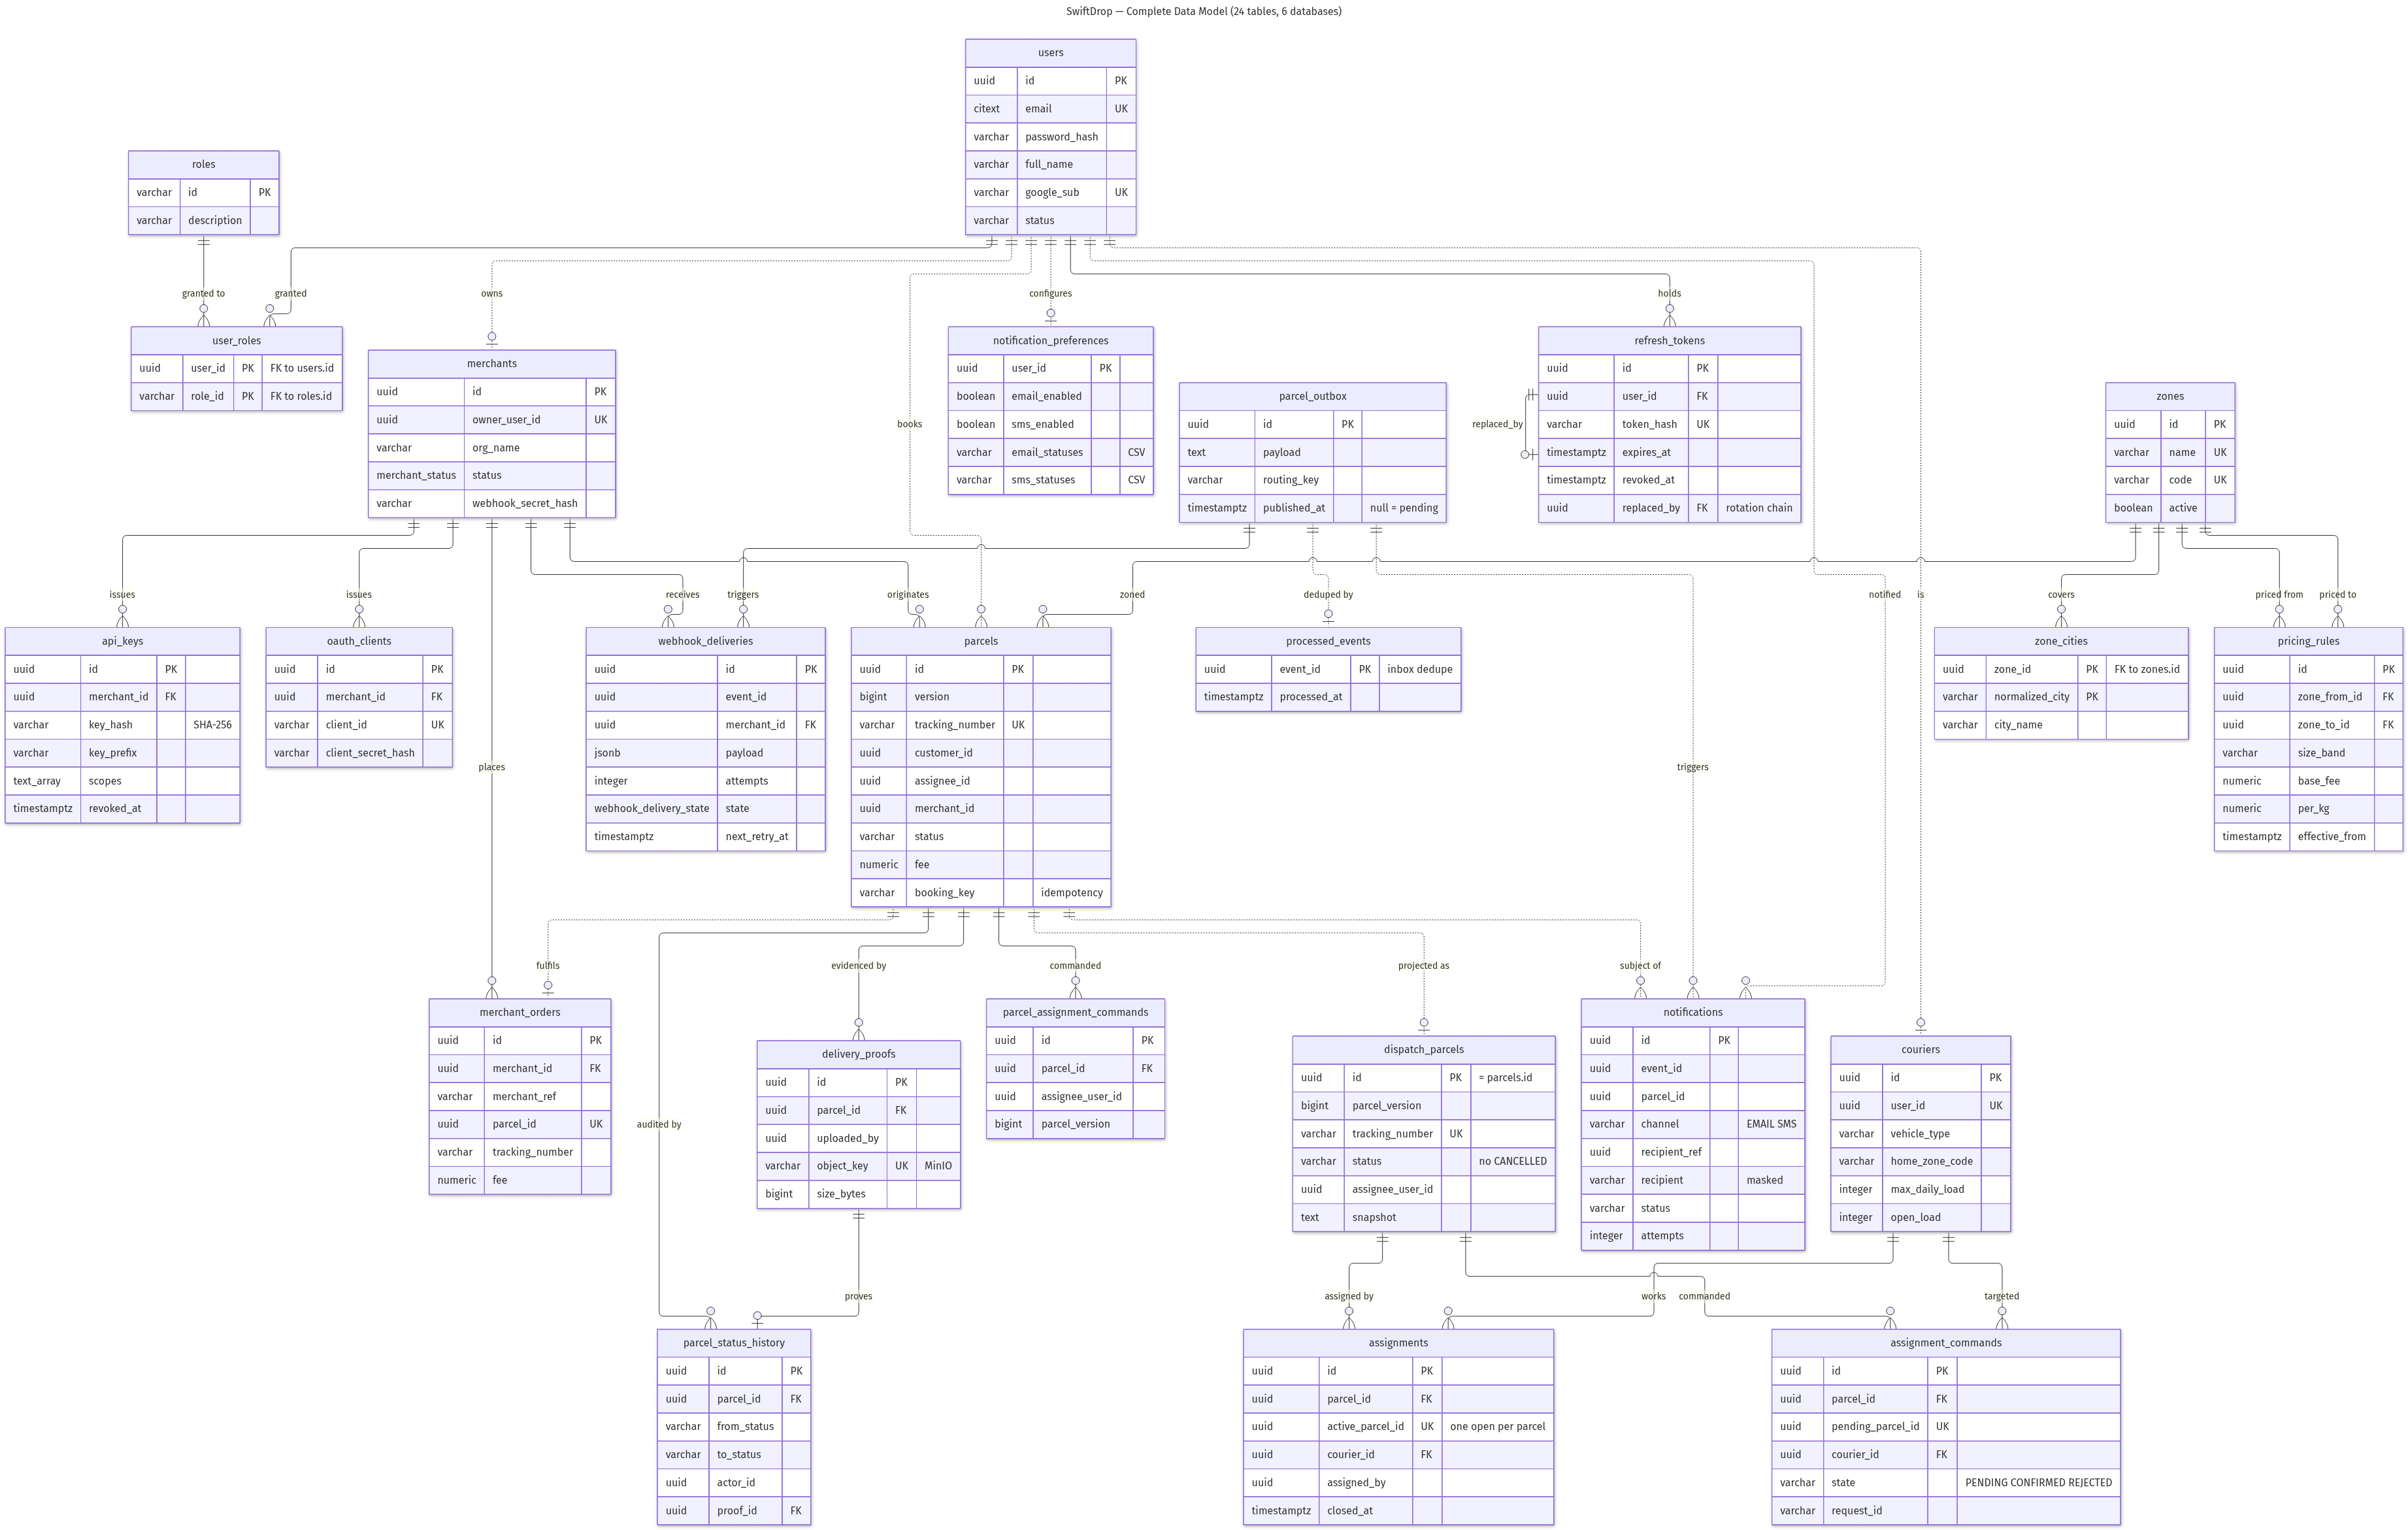
\includegraphics[width=\linewidth,height=0.93\textwidth,keepaspectratio]{er-02-full.png}
  \captionof{figure}{Complete 24-table data model, including the infrastructure tables that make
  the asynchronous integration safe: the transactional outbox, the inbox deduplication table, the
  webhook delivery log and the assignment command tables}\label{fig:er02}
  \end{minipage}}
\end{center}
\clearpage

\subsection{Known Model Drift}
Two asymmetries are visible in the migrations and are recorded here rather than smoothed over:
\begin{enumerate}[leftmargin=*]
\item \code{dispatch\_parcels.status} carries a check constraint rejecting \code{CANCELLED}, while
\code{parcels.status} accepts it, so a cancelled parcel cannot be projected into the dispatch read
model.
\item \code{parcels.pickup\_zone} is \code{VARCHAR(80)} while its logical source
\code{zones.code} is \code{VARCHAR(12)} - the consumer's column is wider than the producer's.
\end{enumerate}

%==============================================================================
\chapter{Integration Architecture and Messaging}

\section{Integration Patterns}
\begin{center}
\small
\begin{longtable}{@{}p{3.3cm}p{5.0cm}p{6.0cm}@{}}
\toprule
\textbf{Pattern} & \textbf{Where used} & \textbf{Why this pattern} \\
\midrule
\endfirsthead
\toprule
\textbf{Pattern} & \textbf{Where used} & \textbf{Why this pattern} \\
\midrule
\endhead
Request/reply & parcel $\rightarrow$ pricing; dispatch $\rightarrow$ identity and parcel;
gateway $\rightarrow$ all & The caller cannot proceed without the answer: a parcel cannot be
persisted before an authoritative fee exists \\
\addlinespace
Publish/subscribe & \code{parcel.events} topic exchange: one producer, four consumers & A status
change has several independent audiences; the producer should not know who they are \\
\addlinespace
Message broker & RabbitMQ topic exchange plus \code{swiftdrop.dlx} & Durable, routable fan-out
with retry and dead-lettering \\
\addlinespace
Transactional outbox & \code{parcel\_outbox} written inside the business transaction, drained by
a scheduled publisher & Removes the dual-write problem: state change and publish intent commit
atomically \\
\addlinespace
Idempotent consumer & \code{processed\_events}; a Redis key with TTL; a unique constraint on
event, channel and recipient & Publisher confirms give at-least-once delivery, so every consumer
must tolerate replay \\
\addlinespace
Idempotency key & \code{Idempotency-Key} header on booking; deterministic key for merchant orders
& A retried booking returns the original parcel rather than creating a duplicate \\
\addlinespace
CQRS read model & \code{dispatch\_parcels}; the Redis tracking projection & Fast reads in a
different shape from the write model, without querying the owning service \\
\addlinespace
API gateway / BFF & Spring Cloud Gateway and the dashboard fan-out & One edge for authentication,
CORS, rate limiting and circuit breaking \\
\addlinespace
Circuit breaker & Resilience4j on every gateway route & Prevents a sick upstream from cascading \\
\addlinespace
Client credentials & \code{POST /api/v1/auth/service-token} & Internal calls authenticate as a
service, carrying no human roles \\
\addlinespace
Token forwarding & parcel $\rightarrow$ pricing; assistant $\rightarrow$ parcel and pricing &
Preserves the user's own authorisation instead of escalating to a service identity \\
\addlinespace
Outbound webhook & merchant-service to the merchant endpoint, HMAC-signed & Push integration for
partners who cannot poll \\
\addlinespace
Fallback ladder & STOMP over WebSocket $\rightarrow$ SSE $\rightarrow$ 15-second polling & Live
updates must survive proxies that break WebSockets \\
\bottomrule
\caption{Integration patterns and the rationale for each}\label{tab:patterns}
\end{longtable}
\end{center}

\diagram{int-01-patterns-map.png}{Integration patterns map. Thick solid edges are synchronous
request/reply; dashed edges are asynchronous publish/subscribe through the broker}{fig:int01}

\section{Messaging Topology and Delivery Guarantees}
Every message is wrapped in a common envelope, \code{EventEnvelope<T>}, carrying \code{eventId},
\code{eventType}, \code{version}, \code{occurredAt}, \code{producer} and the payload. The
\code{eventId} is the deduplication key every consumer uses.

Naming is mechanical: routing keys are \code{<eventType>.v<version>} and queues are
\code{<consuming-service>.<routing-key>}, with \code{.dlq} appended for dead letters. Reading a
queue name reveals both its consumer and its payload.

\begin{center}
\small
\begin{tabular}{@{}p{4.3cm}p{5.4cm}p{4.3cm}@{}}
\toprule
\textbf{Routing key} & \textbf{Queue} & \textbf{Consumer} \\
\midrule
\code{parcel.dispatch.changed.v1} & \code{dispatch.parcel.dispatch.changed.v1} & dispatch-service \\
\addlinespace
\code{parcel.status.changed.v2} & \code{tracking.parcel.status.changed.v2} & tracking-service \\
\addlinespace
\code{parcel.status.changed.v2} & \code{notification.parcel.status.changed.v2} &
notification-service \\
\addlinespace
\code{parcel.status.changed.v2} & \code{merchant-webhook.parcel.status.changed.v2} &
merchant-service \\
\bottomrule
\end{tabular}
\captionof{table}{Bound queues on the \code{parcel.events} topic exchange}\label{tab:queues}
\end{center}

\begin{factbox}
A version~1 status event (\code{parcel.status.changed.v1}) is declared in the shared contracts
module but is \emph{never bound or consumed}. Version~2 is the event actually produced. Note also
that dispatch-service consumes a different event entirely - \code{parcel.dispatch.changed.v1} -
rather than the status event.
\end{factbox}

The guarantee is \textbf{at-least-once}. The producer writes the outbox row inside the business
transaction; the publisher sends persistently and waits for a broker confirmation before marking
the row published; on a negative acknowledgement or return it stops the batch and leaves the row
for the next cycle. Duplicates are therefore possible by design, which is why every consumer
deduplicates.

\diagram{int-02-event-topology.png}{Event topology from the transactional outbox through the topic
exchange to the four bound queues and the dead-letter exchange}{fig:int02}

%==============================================================================
\chapter{Core Workflows and State Transitions}

\section{Customer Booking and Dynamic Pricing}
Two aspects deserve attention. First, the fee is quoted twice - once for display while the
customer types, and again authoritatively inside the booking transaction, so the browser's number
is never trusted. Second, four writes and two outbox rows commit in a single local transaction, so
an event can never be published for a parcel that failed to save, and a saved parcel can never
silently fail to notify.

\diagram{seq-01-create-delivery.png}{Customer booking: debounced estimate, server-side re-quote,
atomic persistence with the transactional outbox, and asynchronous fan-out}{fig:seq01}

\section{Merchant Order Creation via the REST API}
The server-to-server path. The API key is never stored - only its SHA-256 hash and an
eight-character prefix. Verification looks candidates up by prefix, filters by expiry and scope,
and compares hashes in constant time to avoid leaking information through response timing.

Because no user is present, merchant-service obtains a short-lived service token from
identity-service before calling parcel-service. The idempotency key it sends is
\emph{deterministic}, derived from the merchant identifier and the merchant's own reference, so a
retry from the partner's system reuses the same parcel rather than creating a second one.

\diagram{seq-02-merchant-api-order.png}{Merchant REST API order ingestion with API key
verification, service-token acquisition and deterministic idempotency}{fig:seq02}

\section{Courier Status Update Triggering Notifications}
The clearest illustration of the publish/subscribe design: one status update fans out to three
unrelated consumers, none of which the courier's request waits for.

Two deliberate orderings are visible. Proof of delivery is uploaded \emph{before} the status
change, so a failed upload leaves the parcel untouched and the courier simply retries. The
notification recipient is taken from the event's \code{customerUserId} - the parcel's owner - not
from the courier who triggered the change.

\begin{factbox}
Proof-of-delivery objects are uploaded to MinIO by \textbf{parcel-service}, which owns the
\code{ProofStorage} abstraction. Dispatch-service is not involved in the upload path.
\end{factbox}

\diagram{seq-03-status-update-notification.png}{Courier status update fanning out to the
notification pipeline, the tracking projection and the merchant webhook}{fig:seq03}

\section{Google OAuth 2.0 Login with PKCE}
Authorization Code flow with PKCE. The browser is a public client and cannot hold a secret, so
PKCE binds the authorisation code to the client that requested it: the application generates a
random verifier, transmits only its SHA-256 hash, and must present the original verifier to redeem
the code.

The defences worth naming are that \code{state} is single-use and consumed atomically from Redis;
the verifier is compared in constant time; the redirect URI is re-checked against the one recorded
at authorisation time; and the identity token's issuer and audience are verified before any
account is touched. An account provisioned through Google receives a null password hash, so
password login against it can never succeed.

\diagram{seq-04-oauth-login.png}{Google OAuth 2.0 PKCE login, including token exchange,
account link-or-provision, and refresh-token rotation with replay detection}{fig:seq04}

\section{Parcel Lifecycle State Machine}
Transitions are validated against a single declarative table in \code{ParcelStateMachine} rather
than scattered conditionals.

\begin{center}
\small
\begin{tabular}{@{}llp{7.2cm}@{}}
\toprule
\textbf{From} & \textbf{Permitted to} & \textbf{Guard} \\
\midrule
\code{CREATED}          & \code{PICKED\_UP}, \code{CANCELLED} & Cancellation is legal only here \\
\code{PICKED\_UP}       & \code{IN\_TRANSIT}        & - \\
\code{IN\_TRANSIT}      & \code{OUT\_FOR\_DELIVERY} & - \\
\code{OUT\_FOR\_DELIVERY} & \code{DELIVERED}, \code{FAILED} & \code{DELIVERED} requires a
\code{proofId} belonging to this parcel; \code{FAILED} requires a reason \\
\code{FAILED}           & \code{OUT\_FOR\_DELIVERY} & Reattempt \\
\code{DELIVERED}        & - & Terminal; enables receipt download \\
\code{CANCELLED}        & - & Terminal \\
\bottomrule
\end{tabular}
\captionof{table}{Permitted parcel state transitions}\label{tab:states}
\end{center}

\begin{factbox}
\textbf{\code{FAILED} is not a terminal state.} A failed delivery returns to
\code{OUT\_FOR\_DELIVERY} for a reattempt, so the transition graph contains a cycle and the
progression is not strictly linear. Only \code{DELIVERED} and \code{CANCELLED} are terminal.
\end{factbox}

\diagram{act-01-parcel-lifecycle.png}{Parcel lifecycle state machine transcribed from the
implementation, including the failure-reattempt cycle}{fig:act01}

%==============================================================================
\chapter{AI Assistant Service}

\section{Architecture}
SwiftDrop includes an AI assistant service built on Spring AI. A large language model is given a
set of callable domain tools; the model decides which to invoke in response to a natural-language
prompt, and the service streams both its reasoning and each tool invocation back to the browser
over Server-Sent Events.

The service is stateless with respect to durable storage: conversations are held in memory with a
24-hour expiry and are scoped to the calling user.

\section{Implemented Tools}
\begin{center}
\small
\begin{tabular}{@{}p{3.1cm}p{2.3cm}p{8.4cm}@{}}
\toprule
\textbf{Tool} & \textbf{Status} & \textbf{Behaviour} \\
\midrule
\code{estimateFee}   & \Impl & Calls pricing-service to quote a fee from origin, destination, size
band, weight and express flag \\
\addlinespace
\code{trackParcel}   & \Impl & Retrieves the tracking timeline for a tracking number, returning a
privacy-reduced view without contact or street-address detail \\
\addlinespace
\code{listMyParcels} & \Impl & Lists the authenticated customer's own parcels; injected only when
the caller holds the customer role \\
\bottomrule
\end{tabular}
\captionof{table}{Tools currently exposed to the model}\label{tab:aitools}
\end{center}

All three are read-oriented. The assistant can answer questions about the system but cannot
presently modify state.

\section{Designed but Not Yet Implemented}
The following capabilities were designed as part of the agentic vision and are retained here as
roadmap items. None is currently callable.

\begin{center}
\small
\begin{tabular}{@{}p{3.6cm}p{2.3cm}p{7.9cm}@{}}
\toprule
\textbf{Capability} & \textbf{Status} & \textbf{Intended behaviour} \\
\midrule
\code{createParcel} & \Planned & Parse a conversational booking instruction and persist a parcel
end to end, returning a tracking number \\
\addlinespace
\code{assignParcel}, \code{inspectWorkload} & \Planned & Evaluate the unassigned queue and courier
capacity, then propose or trigger assignments \\
\addlinespace
\code{generateApiKey}, \code{retryWebhook} & \Planned & Allow merchants to provision keys and
re-drive failed webhook deliveries conversationally \\
\addlinespace
MCP server exposure & \Partial & The MCP starter dependency is declared, but no server wiring
exists; the tools are not yet reachable over the Model Context Protocol \\
\addlinespace
General per-authority tool filtering & \Partial & A single-role check currently gates
\code{listMyParcels}; a caller holding several roles loses that tool \\
\bottomrule
\end{tabular}
\captionof{table}{Planned assistant capabilities retained in the roadmap}\label{tab:aiplanned}
\end{center}

\section{Security of the Tool Path}
When the model invokes a tool, the service propagates the caller's original bearer token to the
downstream microservice. Existing Spring Security authorisation therefore applies unchanged - the
assistant cannot read anything the user could not read directly through the API. Tool invocations
are streamed to the client before execution, giving the user visibility of exactly what the
assistant is doing on their behalf.

%==============================================================================
\chapter{Design Patterns and Engineering Principles}

\section{Strategy Pattern in the Pricing Engine}
The clearest pattern application in the codebase. \code{PricingEngine} depends only on the
\code{PricingStrategy} interface and receives every implementation as an injected list, sorted by
each strategy's declared order. Calculation reduces over that list, threading a breakdown through
each strategy in turn.

\begin{center}
\small
\begin{tabular}{@{}llp{8.0cm}@{}}
\toprule
\textbf{Strategy} & \textbf{Order} & \textbf{Contribution} \\
\midrule
\code{ZoneBandStrategy}        & 10 & Sets the base fee from the matched pricing rule \\
\code{WeightSurchargeStrategy} & 20 & Charges only weight above the rule's included allowance \\
\code{ExpressSurchargeStrategy}& 30 & Adds the configured express percentage \\
\bottomrule
\end{tabular}
\captionof{table}{Ordered pricing strategy chain}\label{tab:strategies}
\end{center}

Introducing a fuel surcharge means adding one Spring component and nothing else: the engine does
not change, and neither does any existing strategy. The same shape appears again in
notification-service, where a channel router selects from an injected list of channel handlers.

\diagram{pat-01-pricing-strategy.png}{Strategy pattern in the pricing engine}{fig:pat01}

\section{SOLID Principles}
\begin{center}
\small
\begin{longtable}{@{}p{3.3cm}p{10.9cm}@{}}
\toprule
\textbf{Principle} & \textbf{Evidence in the codebase} \\
\midrule
\endfirsthead
\toprule
\textbf{Principle} & \textbf{Evidence in the codebase} \\
\midrule
\endhead
Single responsibility & One bounded context per service; within each, controllers handle HTTP,
services hold rules, repositories handle persistence \\
\addlinespace
Open/closed & The pricing engine and the notification channel router accept new behaviour without
modification \\
\addlinespace
Liskov substitution & Every \code{PricingStrategy} is interchangeable; the engine makes no
assumption about which concrete strategy it holds \\
\addlinespace
Interface segregation & \code{PricingStrategy} declares two methods; \code{ProofStorage} exposes
only what parcel-service needs, which is what makes the MinIO backend swappable \\
\addlinespace
Dependency inversion & High-level policy depends on abstractions the framework satisfies: the
engine on the strategy interface, services on Spring Data interfaces, and parcel-service on a
pricing client interface rather than on an HTTP client \\
\bottomrule
\caption{SOLID principles as applied}\label{tab:solid}
\end{longtable}
\end{center}

\section{Further Patterns Applied}
\begin{center}
\small
\begin{longtable}{@{}p{3.6cm}p{4.6cm}p{6.1cm}@{}}
\toprule
\textbf{Pattern} & \textbf{Implementation} & \textbf{Purpose} \\
\midrule
\endfirsthead
\toprule
\textbf{Pattern} & \textbf{Implementation} & \textbf{Purpose} \\
\midrule
\endhead
State machine & \code{ParcelStateMachine} & Legal transitions declared once in a table a reader
can verify at a glance \\
\addlinespace
Repository & Spring Data JPA interfaces & Business code expresses intent rather than SQL \\
\addlinespace
Transactional outbox & \code{OutboxEvent} and a scheduled publisher & Atomic state change and
event intent \\
\addlinespace
Observer / publish-subscribe & AMQP listeners & Services react to parcel events without the
producer knowing them \\
\addlinespace
Chain of responsibility & Spring Security filter chains; the API key filter ahead of the JWT
filter & A request passes through independent, individually testable concerns \\
\addlinespace
Projection & The dispatch projector and the Redis tracking repository & Read models shaped for
their consumer and reduced for privacy \\
\addlinespace
Data transfer object & View records at every boundary & Entities never serialise directly, so the
wire contract is deliberate and PII can be excluded \\
\addlinespace
Value object & Tracking number; the embeddable address & Validity enforced at construction \\
\addlinespace
Optimistic locking & Version columns on parcel, courier, assignment and pricing rule & Concurrent
edits conflict loudly instead of silently overwriting \\
\bottomrule
\caption{Design patterns applied across the platform}\label{tab:patterns2}
\end{longtable}
\end{center}

\section{Don't Repeat Yourself}
A shared contracts module is the single place where cross-service contracts live: event payload
records, the event envelope, exchange and queue constants, the shared role, status and size
enumerations, and the error-code catalogue behind RFC 7807 responses. Queue names are
\emph{derived} from routing keys rather than written twice, and golden-file tests pin each event's
JSON shape so a field rename that would break a consumer fails the producer's build.

The limit is worth stating: this holds for anything expressible as shared Java, but not for
configuration. The JWT decoder setup is repeated in all eight services, and the claim-name defect
in Section~\ref{sec:defects} is exactly the kind of error that duplication permits.

%==============================================================================
\chapter{Security Architecture}

\section{Cryptographic Authentication}
\begin{center}
\small
\begin{tabular}{@{}p{4.3cm}p{9.9cm}@{}}
\toprule
\textbf{Control} & \textbf{Implementation} \\
\midrule
Token signing & RSA 2048-bit, RS256, key identifier \code{swiftdrop-v1} \\
\addlinespace
Key discovery & RFC 7517 JWKS published at \code{/.well-known/jwks.json}, cached 24 hours;
resource servers validate locally without contacting the identity database \\
\addlinespace
Access token lifetime & 15 minutes \\
\addlinespace
Refresh token & 7 days, opaque, stored only as a SHA-256 digest, rotated on every use \\
\addlinespace
Replay detection & Presenting an already-rotated token revokes the entire token family for that
user \\
\addlinespace
Cookie transport & \code{HttpOnly}, \code{Secure}, \code{SameSite=Strict}, path-scoped to the
authentication endpoints \\
\bottomrule
\end{tabular}
\captionof{table}{Authentication controls}\label{tab:authn}
\end{center}

\section{Defence in Depth}
\begin{center}
\small
\begin{longtable}{@{}p{4.3cm}p{9.9cm}@{}}
\toprule
\textbf{Control} & \textbf{Implementation} \\
\midrule
\endfirsthead
\toprule
\textbf{Control} & \textbf{Implementation} \\
\midrule
\endhead
Password hashing & BCrypt at work factor 10 with a secure random salt \\
\addlinespace
Credential enumeration & A missing email still executes a constant-time dummy verification, and
invalid email and invalid password return an identical problem document \\
\addlinespace
Rate limiting & Redis token buckets at the edge: 5 requests per minute on login, 30 per minute on
public tracking, 100 per minute on other API routes. Keyed by user when authenticated, by address
otherwise, and fails open if Redis is unreachable \\
\addlinespace
API key storage & SHA-256 hash and an eight-character prefix only; verification compares in
constant time \\
\addlinespace
Proof-of-delivery access & MinIO presigned URLs valid for 300 seconds \\
\addlinespace
PII protection & Recipient addresses masked in the notification log; a log converter redacts
emails and phone numbers across all logger statements; the tracking projection excludes addresses
and phone numbers by construction \\
\addlinespace
Identity header integrity & The gateway strips any client-supplied identity header and re-derives
it from a validated token \\
\addlinespace
Transport hardening & CORS allowlist, \code{X-Frame-Options}, \code{nosniff}, HSTS and a content
security policy at the edge \\
\bottomrule
\caption{Defence-in-depth controls}\label{tab:defence}
\end{longtable}
\end{center}

%==============================================================================
\chapter{Quality Assurance and Defect Transparency}

\section{Testing Strategy}
\begin{center}
\small
\begin{tabular}{@{}p{3.6cm}p{2.3cm}p{7.9cm}@{}}
\toprule
\textbf{Tier} & \textbf{Status} & \textbf{Coverage} \\
\midrule
Unit & \Impl & JUnit 5 and Mockito over the pricing strategies, parcel state machine and webhook
retry policy \\
\addlinespace
Integration & \Impl & Testcontainers providing real PostgreSQL and RabbitMQ for repository and
messaging tests \\
\addlinespace
Authorisation & \Impl & \code{RbacAuthorizationIntegrationTest},
\code{DispatchAuthorizationTest} and \code{PricingAuthorizationTest} assert that unauthorised
roles are refused and that spoofed identity headers are rejected \\
\addlinespace
Concurrency & \Impl & \code{AssignmentConcurrencyTest} proves capacity limits and unique-assignment
protection against a real database \\
\addlinespace
Contract & \Impl & Golden-file tests pin every event's JSON shape in the shared contracts module \\
\addlinespace
API & \Impl & Spring MockMvc and WebTestClient slices \\
\addlinespace
End-to-end browser & \Planned & Playwright smoke tests are specified but not present in the web
application manifest \\
\bottomrule
\end{tabular}
\captionof{table}{Testing tiers and status}\label{tab:testing}
\end{center}

\section{Defect Audit}\label{sec:defects}
Verifying this report against the implementation surfaced six defects. They are recorded here
because the diagrams in this document depict the system as it actually behaves.

\begin{enumerate}[leftmargin=*]
\item \textbf{JWT claim name mismatch.} identity-service writes the merchant claim as
\code{merchantId}; parcel-service, the gateway identity filter and tracking-service all read
\code{merchant\_id}. Merchant-scoped operations performed with a user token cannot resolve a
merchant.

\item \textbf{Dead bearer-token branch in merchant order creation.} The controller tests whether
the authentication object is a \code{Jwt}, but it is a \code{JwtAuthenticationToken} whose
\emph{principal} is the \code{Jwt}. The test never passes, so even a console-originated merchant
order falls through to the service-token path. Functionally benign today; incorrect as written.

\item \textbf{API-key requests cannot traverse the gateway.} The gateway security chain is
JWT-only and has no API-key filter, so a request carrying an API key is refused at the edge. The
documented merchant integration therefore works only against merchant-service directly, which is
how Figure~\ref{fig:seq02} draws it.

\item \textbf{Unauthenticated internal identity lookup.} notification-service calls the internal
user lookup with no authorisation header. The endpoint requires a scoped service token, so the
call fails and a catch-all fallback substitutes a synthetic placeholder address rather than
failing loudly.

\item \textbf{Dashboard aggregates endpoints that do not exist.} The gateway BFF endpoint calls a
summary route on parcel, dispatch and merchant services. No such route is implemented on any of
them, so the dashboard always returns unavailable sections.

\item \textbf{Public tracking detail endpoint is not public.} The web application calls a parcel
detail-by-tracking route as though anonymous, but parcel-service permits only the summary route
without authentication.
\end{enumerate}

\section{Consolidated Implementation Status}\label{sec:statusmatrix}
\begin{center}
\small
\begin{longtable}{@{}p{6.4cm}p{2.3cm}p{5.1cm}@{}}
\toprule
\textbf{Capability} & \textbf{Status} & \textbf{Remark} \\
\midrule
\endfirsthead
\toprule
\textbf{Capability} & \textbf{Status} & \textbf{Remark} \\
\midrule
\endhead
Identity, RBAC, JWT, JWKS, Google OAuth PKCE & \Impl & Including refresh rotation and replay
revocation \\
Zone-based pricing with Strategy engine & \Impl & Temporal rules with overlap protection \\
Parcel booking, state machine, receipts & \Impl & Idempotent booking \\
Proof-of-delivery capture to object storage & \Impl & Presigned retrieval \\
Courier dispatch, assignment, workload & \Impl & Command-based with compare-and-set \\
Merchant onboarding, API keys, orders & \Impl & Scoped keys, hashed at rest \\
Outbound signed webhooks with retry & \Impl & Exponential backoff to one hour \\
Real-time tracking ladder & \Impl & STOMP, SSE, polling \\
Email notification pipeline & \Impl & Preference-aware, idempotent \\
SMS notification channel & \Partial & Mock provider only \\
AI assistant read tools & \Impl & Three tools \\
AI assistant write/automation tools & \Planned & Booking, dispatch, merchant operations \\
MCP server exposure & \Partial & Dependency declared, wiring absent \\
Volumetric dimension pricing & \Planned & Size bands today \\
Merchant volume discounts & \Planned & No discount logic \\
Recipient-addressed notifications & \Planned & Owner-addressed today \\
Docker Compose local orchestration & \Impl & Full stack \\
Playwright end-to-end tests & \Planned & Not in the manifest \\
\bottomrule
\caption{Consolidated implementation status matrix}\label{tab:statusmatrix}
\end{longtable}
\end{center}

%==============================================================================
\chapter{Team Contributions and Project Management}

\section{Work Breakdown}
\begin{center}
\small
\begin{longtable}{@{}p{2.0cm}p{3.4cm}p{2.9cm}p{5.1cm}@{}}
\toprule
\textbf{Index} & \textbf{Member} & \textbf{Area} & \textbf{Key contributions} \\
\midrule
\endfirsthead
\toprule
\textbf{Index} & \textbf{Member} & \textbf{Area} & \textbf{Key contributions} \\
\midrule
\endhead
234021D & Arangala A. P. & Identity \& Auth & RS256 token service, JWKS endpoint, Google OAuth
PKCE, refresh rotation, RBAC test suite \\
\addlinespace
        & Kevin Gaveshana & Gateway \& Edge & Spring Cloud Gateway routes, Redis rate limiting, circuit
breakers, Docker Compose infrastructure \\
\addlinespace
234127H & M.A.P.M. Mallawasekara & Pricing \& Zones & Strategy chain, zone and city resolution, temporal pricing
rules \\
\addlinespace
234087H & L. P. Ishadi & Parcel Lifecycle & Parcel state machine, tracking number generation,
receipt generation, transactional outbox \\
\addlinespace
234149C & Methsara & Dispatch \& Couriers & Courier roster, workload accounting,
assignment commands, proof-of-delivery upload \\
\addlinespace
        & Charithma Dassanayake & Merchant API & API key lifecycle, order ingestion, HMAC-signed
webhooks with retry and dead-lettering \\
\addlinespace
234009A & Maheesha Paboth & Live Tracking & STOMP over SockJS, SSE fallback, Redis projection,
public tracking timeline \\
\addlinespace
234208H & Thranjaya S. J. K. & Notifications & AMQP consumer, Mailpit integration, Thymeleaf
templates, preference engine, PII masking \\
\addlinespace
234234H & R.K.T.P. Wijerathna & AI Assistant & Spring AI integration, tool callbacks, SSE
streaming of tool invocations \\
\addlinespace
234035A & K.G.T. Buddhima & Frontend \& Design & React SPA for all four personas, realtime
transport ladder, verified architecture documentation and the eighteen diagrams in this report \\
\bottomrule
\caption{Ten-member work breakdown}\label{tab:team}
\end{longtable}
\end{center}

\section{Milestone Progression}
\begin{description}[leftmargin=1.9cm,style=sameline]
\item[M1 - Foundation] Multi-module Maven aggregator, database schemas, gateway routing, JWKS
validation.
\item[M2 - Core flows] Registration, Google OAuth, fee calculation, parcel booking.
\item[M3 - Events] RabbitMQ pipeline, courier assignment, live tracking, email notification.
\item[M4 - Partner \& admin] Merchant API keys, order ingestion, webhook delivery, admin
consoles.
\item[M5 - Hardening] Testcontainers integration tests, RBAC suites, and the verified design
documentation on which this report is based.
\end{description}

%==============================================================================
\chapter{Conclusion and Roadmap}

\section{Conclusion}
SwiftDrop demonstrates that a microservice architecture with an API gateway, database-per-service
isolation, and event-driven integration delivers meaningful decoupling and resilience for a
logistics domain. The implementation applies recognised patterns - transactional outbox, idempotent
consumers, CQRS projections, Strategy-based pricing, circuit breaking and asymmetric
authentication - and backs them with an automated test suite including real-infrastructure
integration tests.

The report is deliberate about what is not finished. Two substantial items, browser end to end
testing and the write capable AI tooling, remain designed rather than delivered, and six defects
found during verification are recorded in
Section~\ref{sec:defects}. Documenting these alongside the working system is a more useful
engineering artefact than a report that claims uniform completeness.

\section{Roadmap}
\begin{enumerate}[leftmargin=*]
\item \textbf{Close the six recorded defects}, beginning with the JWT claim-name mismatch, which
silently disables merchant-scoped operations.
\item \textbf{Add Playwright end-to-end smoke tests} covering booking, courier status update and
public tracking.
\item \textbf{Extend the AI assistant with write-capable tools} - booking, dispatch assignment and
merchant operations - behind per-authority tool filtering, and complete the MCP server wiring.
\item \textbf{Introduce volumetric pricing and merchant volume discounts} as additional strategies
in the existing ordered chain, which requires no change to the pricing engine.
\item \textbf{Address the recipient} as well as the sender in the notification pipeline.
\item \textbf{Integrate a production SMS provider} behind the existing channel abstraction.
\item \textbf{Longer term:} route optimisation, native courier mobile clients with offline sync,
and payment gateway integration for merchant billing and cash-on-delivery reconciliation.
\end{enumerate}

\end{document}
